% Cover letter: Application Engineer - 3D Metrology, ZEISS (Trnava)
% CV: Sections/cv_zeiss_metrology.tex -> cv_gen/cv_giovanni_tauro-zeiss.pdf
\documentclass[11pt,a4paper,sans]{moderncv}
% Shared preamble and header for the cover letters.
% One main file per application: cl_<company>.tex, built to
% cv_gen/coverletter_giovanni_tauro-<company>.pdf next to cv_giovanni_tauro-<company>.pdf.
% Paths (cl_gen/..., Pictures/...) are relative to the project root, as in the CV (see .latexmkrc).

\moderncvstyle{classic}
\moderncvcolor{blue}

\usepackage[scale=0.80]{geometry}
\setlength{\footskip}{136.00005pt}

\usepackage{fontawesome5}
% hyperref is loaded by moderncv itself; loading it here causes an option clash
\usepackage{xcolor}
\usepackage{graphicx}
\ifxetexorluatex
  \usepackage{fontspec}
  \usepackage{unicode-math}
  \defaultfontfeatures{Ligatures=TeX}
  \setmainfont{Latin Modern Roman}
  \setsansfont{Latin Modern Sans}
  \setmonofont{Latin Modern Mono}
  \setmathfont{Latin Modern Math}
\else
  \usepackage[T1]{fontenc}
  \usepackage{lmodern}
\fi

\usepackage[english]{babel}

% used for the PDF title and the letter closing; the visible header is \clheader below
\name{Giovanni}{Tauro}

% Header: #1 = headline under the name (same as the headline of the matching CV)
\newcommand{\clheader}[1]{%
\noindent
\begin{minipage}[c]{0.74\textwidth}
    {\Huge \textbf{Giovanni Tauro}}\\[-0.2em]
    {\small #1}\\[0.3em]

    \footnotesize
    \faMapMarker*~
    \href{https://www.google.com/maps/search/?api=1&query=Lecco+23900+Italy}
    {\color{blue}Bari-Lecco, Italy}
    \quad
    \faPhone*~
    \href{https://wa.me/393279437161}
    {\color{blue}+39 3279437161}
    \quad
    \faEnvelope~
    \href{mailto:giovanni.taurodi@gmail.com}
    {\color{blue}giovanni.taurodi@gmail.com}
    \\[-0.1em]

    \faLinkedin~
    \href{https://www.linkedin.com/in/giovanni-tauro-gt/}
    {\color{blue}LinkedIn}
    \quad
    \faGithub~
    \href{https://github.com/jotades}
    {\color{blue}GitHub}
    \quad
    \faGraduationCap~
    \href{https://scholar.google.com/citations?user=BS0aVGgAAAAJ&hl=it}
    {\color{blue}Scholar}
    \quad
    \faFilePdf~
    \href{https://www.notion.so/Giovanni-Tauro-2a7901d92f3a800b892af425c5875c6a}
    {\color{blue}Portfolio}
    \quad
    \faCubes~
    \href{https://grabcad.com/giovanni.tauro-3}
    {\color{blue}GrabCAD}

\end{minipage}
\hfill
\begin{minipage}[c]{0.18\textwidth}
    \raggedleft
    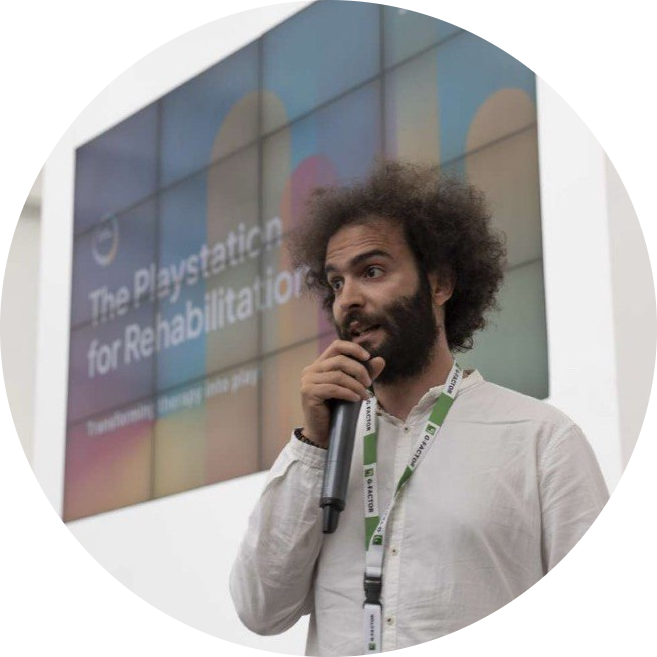
\includegraphics[width=2.8cm]{Pictures/Giovanni_pitch}
\end{minipage}
\vspace{0.1em}
}

\makeatletter
% the sender details are already in \clheader, so skip moderncv's own block
\@detailsfalse
% closing phrase, signature, name
\renewcommand*{\makeletterclosing}{%
  \@closing\\[0.6em]%
  
\includegraphics[height=1.2cm]{Pictures/sign_gt.jpg}\\[0.2em]%
  {\bfseries\@firstname~\@lastname}}
\makeatother


\begin{document}

\clheader{R\&D Engineer | 3D Scanning, Reverse Engineering \& CAD}

\recipient{ZEISS Recruiting Team}{Attn. Abbie Walters\\Trnava, Slovakia}
\opening{Dear Abbie Walters,}
\closing{Sincerely,}
\makelettertitle

I am applying for the Application Engineer -- 3D Metrology position in Trnava. I am an R\&D engineer with a BSc in Industrial Design and an MSc in Design \& Engineering from Politecnico di Milano, and for more than five years I have developed and tested devices at CNR-STIIMA, the Italian National Research Council, and as Head of Product of Rehabilia Technologies. The role combines measurement work, customer requirements and presenting technology to users, and those are the parts of my work I enjoy most.

My first professional work was in 3D scanning and reverse engineering. As a freelancer with DIMA3D, I ran end-to-end workflows for medtech, automotive and extreme-sports clients: acquiring 3D scan data, processing it in Geomagic and rebuilding it as validated parametric models in SolidWorks, ready for manufacturing. Since then I have worked daily with CAD, technical drawings and physical prototypes, designing and 3D printing parts, assembling them and testing them against requirements and evaluation protocols that I designed myself.

A large part of my job is translating between users and engineering. At Rehabilia I collect requirements from clinicians and partners, turn them into technical specifications for engineers and suppliers, and present the device to clinicians, partners and the EIT Health programme. I have also presented my research at conferences and at KUKA Deutschland, so I am comfortable explaining a technical system to people with different backgrounds, which I expect is central to training customers and presenting at trade fairs.

To be transparent, my hands-on experience is with 3D scanning; I have not yet worked with tactile CMMs or CT scanning, nor with ZEISS measurement software. I learn new tools quickly and would welcome the structured training of a company that defines the standard in metrology. I work in English in international projects, including research stays in the Netherlands and Japan.

I would welcome the chance to discuss the role further.

\makeletterclosing

\end{document}
